%%
%% This is file `sample-sigconf.tex',
%% generated with the docstrip utility.
%%
%% The original source files were:
%%
%% samples.dtx  (with options: `sigconf')
%% 
%% IMPORTANT NOTICE:
%% 
%% For the copyright see the source file.
%% 
%% Any modified versions of this file must be renamed
%% with new filenames distinct from sample-sigconf.tex.
%% 
%% For distribution of the original source see the terms
%% for copying and modification in the file samples.dtx.
%% 
%% This generated file may be distributed as long as the
%% original source files, as listed above, are part of the
%% same distribution. (The sources need not necessarily be
%% in the same archive or directory.)
%%
%% The first command in your LaTeX source must be the \documentclass command.
\documentclass[sigconf, nonacm, natbib, screen, balance=False]{acmart}

% Documentation for packages
% - ACM Article Template
%    https://www.acm.org/publications/proceedings-template
% - Pseudocode typesetting CLRS-style:
%    https://www.cs.dartmouth.edu/~thc/clrscode/clrscode3e.pdf
% - Python code typesetting
%    http://ctan.uib.no/macros/latex/contrib/listings/listings.pdf
% - AMS Math
%    http://ctan.uib.no/macros/latex/required/amsmath/amsldoc.pdf
% - Graphics
%    http://ctan.uib.no/macros/latex/required/graphics/grfguide.pdf

\usepackage{clrscode3e}  
\usepackage{listings}
\lstset{language=Python, basicstyle=\ttfamily}
\usepackage{graphicx}

% based on https://tex.stackexchange.com/questions/279240/float-for-lstlisting
\usepackage{float}
\floatstyle{ruled}
\newfloat{listing}{tbph}{lop}
\floatname{listing}{Listing}
\def\lstfloatautorefname{Listing} % needed for hyperref/auroref
\citestyle{acmauthoryear}

%% end of the preamble, start of the body of the document source.
\begin{document}

\pagestyle{plain}

%%
%% The "title" command has an optional parameter,
%% allowing the author to define a "short title" to be used in page headers.
\title{Benchmarking Sorting Algorithms In Python}
\subtitle{INF221 Term Paper, NMBU, Autumn 2020}

\author{Jon-Mikkel Korsvik}
\email{jonkors@nmbu.no}
\affiliation{}  % separates Jane's and Joe's author block

\author{Yva Sandvik}
\email{ysandvik@nmbu.no}

%% The abstract is a short summary of the work to be presented in the
%% article.
\begin{abstract}
  In this paper we analysed and compared the runtime of a selection of sorting algorithms with different problem types. We cover theory and pseudocode, how we created data and plots, what challenges were encountered and the optimizations applied. Finally we discuss how and why hybrid sorting algorithms, such as merge sort combined, are superior sorting algorithms. 
\end{abstract}

%%
%% This command processes the author and affiliation and title
%% information and builds the first part of the formatted document.
\maketitle

\section{Introduction}\label{sec:intro}

Sorting algorithms are used to solve one of the key problems of computer science known as “The sorting problem”. This involves an input sequence of n numbers $a_1, a_2, … , a_n$, where the output is a permutation of the input sequence such that the numbers are ordered in an ascending or descending order. The two main aspects to a sorting algorithm is its time complexity (speed) and its space complexity (memory usage).

During this investigation we have assessed the performance of the sorting algorithms listed below, with certain assumptions regarding their time complexity. We compared their performance using the Python 'time' function, benchmarking their performance when sorting arrays ordered in various ways. In addition we assessed the time-development as the length of the arrays increased.  

\section{Theory}\label{sec:theory}

In the following subsections we will provide theory, pseudocode, as well as details surrounding the methods used when comparing the following sorting algorithms: 

\begin{itemize}

\item Quadratic algorithms
  \begin{itemize}
  \item Insertion sort
  \item Bubble sort
  \end{itemize}
\item Sub-quadratic algorithms
  \begin{itemize}
  \item Merge sort
  \item Quick sort
  \end{itemize}
\item Combined algorithm
  \begin{itemize}
  \item Merge sort switching to insertion sort for small data
  \end{itemize}
\item Built-in sorting functions
  \begin{itemize}
  \item Python 'sort()'
  \item NumPy 'sort()'
  \end{itemize}
\end{itemize}

\subsection{Algorithm 1 - Insertion sort}\label{sec:algo1}
Insertion sort, found in listing ~\ref{lst:insertion_algo}, is a simple in place and comparison based sorting algorithm. Best case run-time for this algorithm is:

\begin{equation}
  T(n) = \Theta(n) \;.  \label{eq:ins_sort_best}
\end{equation}

This is achieved when the input array is already sorted. The worst case run-time occurs if the input list is in reversed order. This gives a quadratic run-time of:

\begin{equation}
  T(n) = \Theta(n^2) \;  \label{eq:ins_sort_worst}
\end{equation}

The average run-time is also quadratic, making insertion sort a bad choice for sorting large lists, however it is one of the best and quickest alternatives when it comes to sorting smaller lists. 

\begin{listing}
  % Pseudocode caption above the code.
  \caption{Insertion sort algorithm from \citet[Ch.~2.1]{CLRS}.}
  \label{lst:insertion_algo}

  \begin{codebox}
    \Procname{$\proc{Insertion\_sort}(A)$}
    \li \For $j \gets 2$ \To $\attrib{A}{length}$
    \li \Do
    $\id{key} \gets A[j]$
    \li     $i \gets j-1$
    \li      \While $i>0$ and $A[i] > \id{key}$
    \li      \Do
    $A[i+1] \gets A[i]$
    \li         $i \gets i-1$
    \End    
    \li       $A[i+1]\gets \id{key}$
    \End
  \end{codebox}
\end{listing}

\subsection{Algorithm 2 - Bubble sort}\label{sec:algo2}

Bubble sort, found in listing~\ref{lst:bubble_algo}, is know as a straightforward and simple sorting algorithm. Both when it comes to implementation and understanding. However its main disadvantage is its inefficiency, especially when sorting large arrays.

Although bubble sort and insertion sort grow asymptotically at the same rate $\Theta(n^2)$, the difference in bubble sort and insertion sort lies in the number of comparisons. In contrast to insertion sort, bubble sort could in the worst case have to make numerous comparisons that do not necessarily result in a swap, making it computationally slower. 

\begin{listing}
  % Pseudocode caption above the code.
  \caption{Bubble sort algorithm from \citet[Ch.~2.1]{CLRS_2009}.}
  \label{lst:bubble_algo}

  \begin{codebox}
    \Procname{$\proc{Bubble\_sort}(A)$}
    \li $n \gets \attrib{A}{length}$
    \li $swapped \gets \id{False}$
    \li $rounds \gets 0$
    \li \While $swapped:$
    \li \Do
    $swapped \gets \id{False}$
    \li \For $i \gets 0 $ \To $\id{n - rounds - 1}$
    \li     \Do
    \If $A[i] > A[i+1]:$
    \li     \Do
    $A[i], A[i+1] \gets A[i+1], A[i]$
    \li $swapped \gets \id{True}$
    \End
    \End    
    \li $rounds + 1$
    \End
  \end{codebox}
\end{listing}


\subsection{Algorithm 3 - Merge Sort}\label{sec:algo3}

Merge sort, found in listing~\ref{lst:merge_algo}, is yet another comparison-based sorting algorithm that uses the divide-and-conquer approach which involves recursively merging together two presorted arrays such that the resulting array also is sorted. Unlike insertion sort and bubble sort it does not iterate through the entire list several times, but instead uses this recursive divide and conquer approach which gives a consistent average and worst case performance of: 

\begin{equation}
  T(n) = \Theta(n\lg n) \;  \label{eq:merge_sort_best}
\end{equation}

This is in fact the best possible run-time that can be achieved by a sorting algorithm. In addition, the fact that the input array is split into subsets, opens for the possibility to sort the two subsets simultaneously, also called to parallelize, which naturally increases the efficiency further.

However, one of merge sorts drawbacks stems from the time cost caused by recursion which effects its performance when sorting smaller lists. In addition, the most common implementations of merge sort do not sort in place. Bringing us to a second drawback of merge sort; its memory requirement. The memory size of the input must be allocated for the sorted output to be sorted in, hence it uses more memory space than other in place sorting algorithms. 

\begin{listing}
  % Pseudocode caption above the code.
  \caption{Merge sort algorithm from \citet[Ch.~2.1]{CLRS_2009}.}
  \label{lst:merge_algo}

  \begin{codebox}
    \Procname{$\proc{Merge\_sort}(A)$} 
    \li \If \attrib{A}{length} > 1: 
    \li \Do
    $mid \gets \attrib{A}{length}$/2: 
    \li $L\_array\gets A[:mid]$
    \li $R\_array\gets A[mid:]$
    \li $\proc{Merge\_sort}(L\_array)$
    \li $\proc{Merge\_sort}(R\_array)$
    \li $L\_index\gets 0$
    \li $L\_index\gets 0$
    \li $copy\_index\gets 0$
    \li \While $L\_index < L\_array$ $and$ $R\_index < R\_array$ 
    \li \Do
    \If $L\_array[L\_index] < R\_array[R\_index]$
    \li \Do
    $L\_index + 1$
    \li \Else:
    \li $A[copy\_index] \gets R\_array[R\_index]$
    \li $R\_index + 1$
    \End
    \End
    \li \While $L\_index < \attrib{L\_array}{length}$
    \li \Do
    $A[copy\_index] \gets L\_array[L\_index]$
    \li $L\_index + 1$
    \li $copy\_index + 1$
    \End
    \li \While $R\_index < \attrib{R\_array}{length}$
    \li \Do
    $A[copy\_index] \gets R\_array[R\_index]$
    \li $R\_index + 1$
    \li $copy\_index + 1$    
  \end{codebox}
\end{listing}

\subsection{Algorithm 4 - Quick sort}\label{sec:algo4}

Quick sort is an efficient and important in place divide-and-conquer sorting algorithm. When implemented well it can supposedly be about two or three times faster than its main competitors, such as merge sort.

It shares the same average time complexity as merge sort, and it is also straightforward to parallelize since it also uses the divide and conquer approach. However the worst case time complexity of quick sort is its main disadvantage, and is $\Theta(n^2)$, i.e no better than insertion sort. This becomes an issue when the input is  an already sorted array, almost sorted array, or reversed sorted array, as quick sort still needs to do several recursions even though the list is sorted or almost sorted. 

The partitioning that occurs when quick sort splits the input array into two subsets is based on a pivot element. The selection of the pivot is critical to the worst case performance of quick sort because it determines the number of necessary recursion levels that will occur. If the algorithm consistently picks the median element as pivot, as opposed to the first, last or a random element, one can guarantee that one will get the best time complexity. Meaning, the worst time complexity can be avoided if the partitioning is balanced, making the expected run-time $\Theta(n\lg n)$, such as merge sort.

In listing~\ref{lst:quick_algo} you can see how we chose to implement the partitioning in quick sort. We used a 'median of three' optimization to handle the worst case scenarios of input arrays that are in ascending or descending order. 

\begin{listing}
  % Pseudocode caption above the code.
  \caption{Quick sort algorithm from \citet[Ch.~2.1]{CLRS_2009}.}
  \label{lst:quick_algo}
  
 \begin{codebox}
    \Procname{$\proc{Median\_of\_three}(A, low, high)$}
    \li mid = (low + high) // 2
    \li \If A[mid] < A[low]
    \li \Do
    exchange A[low] with A[mid]
    \End
    \li \If A[high] < A[low]
    \li \Do
    exchange A[low] with A[high]
    \End
    \li \If A[mid] < A[high]
    \li \Do
    exchange A[mid] with A[high]
  \end{codebox}

  \begin{codebox}
    \Procname{$\proc{Partition}(A, low, high)$}
    \li $\proc{Median\_of\_three}(A, low, high)$
    \li $pivot \gets A[high]$
    \li $i \gets low - 1$
    \li \For $j \gets low $ \To $high -1$ 
    \li \Do
    \If $A[j] \leq pivot$
    \li \Do
    $i \gets i + 1$
    \li exchange A[i] with A[j]
    \End
    \End
    \li exchange A[i + 1] with A[r]
    \li \Return $i +1$
  \end{codebox}

  \begin{codebox}
    \Procname{$\proc{Quick sort}(A, low, high)$}
    \li \If $low < high$
    \li \Do
    $pivot \gets \proc{Partition(A, low, high)}$
    \li $\proc{}(A, low, pivot-1)$
    \li $\proc{Quick sort}(A, pivot+1, high)$
  \end{codebox}

\end{listing}

\subsection{Algorithm 5 - Merge sort combined}\label{sec:algo5}

Merge sort can be optimized to give merge sort combined, found in listing~\ref{lst:mergecombined_algo}, by integrating insertion sort and making it a 'hybrid algorithm'. This takes advantage of the fact that insertion sort performs well on smaller lists. It will therefor use fewer comparisons in the worst case than both merge sort and insertion sort, potentially making it a very efficient sorting algorithm.  

\begin{listing}
  % Pseudocode caption above the code.
  \caption{Merge sort combined algorithm from \citet[Ch.~2.1]{CLRS_2009}.}
  \label{lst:mergecombined_algo}
  
 \begin{codebox}
    \Procname{$\proc{Merge\_sort\_combined}(A, threshold\gets11)$} 
    \li \If $\attrib{A}{length} > threshold$
    \li \Do
    $\proc{Merge\_sort}(A)$
    \li \Else:
    \li $\proc{Insertion\_sort}(A)$
  \end{codebox}
\end{listing}

\subsection{Algorithm 6 - Python "sort()" }\label{sec:algo6}

Since version 2.3 ‘Timsort’ has been the 'built-in' sorting function in Python. In similarity to merge sort combined, timsort is a hybrid sorting algorithm derived from merge sort and insertion sort. \newline
It is a stable sorting algorithm with the a time complexity of $\Theta(n\lg n)$. It starts by using insertion sort to boost the smaller naturally sorted elements found in the unsorted array to a sufficient size, after which they are merged using merge sort. By using insertion sort on the smaller lists one reduces the overhead produced by using more complex algorithms on such small lists. 

The small subsets, also called 'Runs', need to be of a minimum size, often between 32 and 64 elements, however this depends on the length of the array that is to be sorted. 

The Python sort() method does not require any mandatory parameters but offers two optional parameters: 'key' and 'reverse'. The 'key' parameter serves as a key for the comparison. The reverse parameter defines the order. Default being 'False, which denotes ascending order.  

\subsection{Algorithm 7 - NumPy "sort()" }\label{sec:algo7}

NumPy sort() is the 'built-in' NumPy function which sorts an array in-place. NumPy sort() can alternate between three sorting algorithms, the default being quick sort, if specified one can also use merge sort or heap sort. 

The only mandatory input argument to the NumPy sort() function is the input array to be sorted. Otherwise one can choose which axis of the array one wishes to sort, the default is -1. One can choose which algorithm one wants to use (out of the three mentioned above), and lastly one can choose the order one wishes the array to be sorted. Ascending order is the default.

\section{Methods}\label{sec:methods}

\begin{itemize}
\item Our test data is generated using the class function ArrayGenerator found in our utility file.
\item First test data is generated, then our benchmark function times how long each algorithm uses to sort given lists with given lengths.  
\item The timer function times each sorting algorithm in a list a given number of repetitions and returns all the results in a dictionary, as well as printing stats if verbose.
\item Timing data is unpacked as a pandas DataFrame with columns $2^N$, Time, TypeArray and Algorithm . 
\item OS : Windows 10, Python version 3.7.9, 
Processor:	Intel(R) Core(TM) i5-8250U CPU @ 1.60GHz, 1801 Mhz, 4 cores, 8 logic threads.
8 GB of installed RAM. 
\textbf{Make and model:} Huawei MateBook X Pro i5 dGPU 8GB 256GB (2018)

\item Git hashes are provided in table ~\ref{tab:hashes}.
\end{itemize}

\subsection{Data generation - Array Generator}\label{sec:methdata}
We have decided to use a factor of $2^n$ for generating arrays. Giving us binary growth of problem sizes with binary increment benchmarking. 

\subsubsection{Reasoning behind using binary scale.}\label{sec:datareason} This will give us a great range from lists of 1 to lists of 1,073,741,824 elements. In addition the binary scale will reduce the size of results by a factor of. $\frac{n}{a \log_2(n)}$ where $a$ is a scalar representing linear step sizes. The benchmark process shaves of time usage by a factor of $\frac{\sum_{k=1}^{n/a}T\left(k\cdot a \right)}{\sum_{k=1}^{\log_{2}n}T \left(2^{k}\right)}$, where T(x) is the $\mathcal{O}(n)$ of an algorithm. This will ease the computation time for generating data as well as plots while retaining information of the trend in runtimes for every algorithm. 

\subsubsection{Approach.}\label{sec:dataapproach}Using an object oriented approach we can set the seed of a random number generator from NumPy and gather the benefits of large data compared to the standard random library in Python. 
The ArrayGenerator class can create arrays such as shown in figure ~\ref{fig:arrays}. We can create random arrays of both float and integer type. Indicated in later plots as correspondingly \textbf{Random} and \textbf{Integers}. 

\begin{figure}
  \centering
  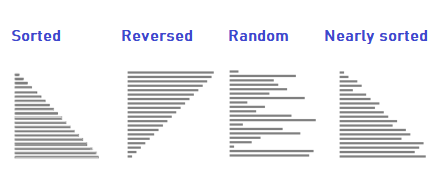
\includegraphics[scale=0.8]{types_of_arrays.PNG}
  % figure captions below figure
  \caption{Different problem types}
  \label{fig:arrays}
\end{figure}

\begin{figure}
  \centering
  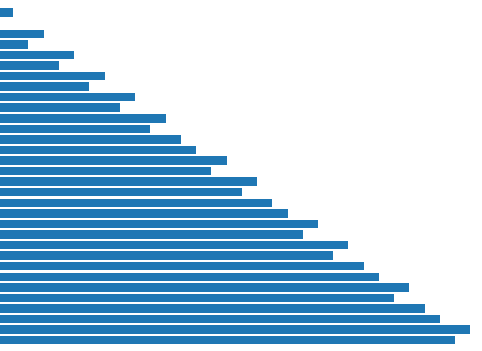
\includegraphics[scale=0.65]{structured array.png}
  % figure captions below figure
  \caption{Structured Array}
  \label{fig:structarr}
\end{figure}

\subsubsection{Creation of the Arrays}\label{sec:createarrays}

Sorted and Reversed are made using NumPy arrange method. Random and Integers are created using the random number generator of the class. The nearly sorted array or the structured array is generated as shown in listing ~\ref{lst:nearlysorted} and gives an array as shown in figure ~\ref{fig:structarr}.


\begin{listing}[h]
  % Listing captions above the listing.   
  \caption{Excerpt from ArrayGenerator in utility.py}
  \label{lst:nearlysorted}
  \begin{lstlisting}
ArrayGenerator.structured_array(self, n):
    """
    Creates array with ascending structure.
    """
    A = np.arange(0, int(2**n))
    
    # Shuffle range
    s_r = int(((2**n))//((n**2)/2))
    
    for i in range(0, int(2**n), s_r):

        #In place shuffle within indices
        self.rng.shuffle(A[i: i + s_r])

    return A.astype('int32')
   
  \end{lstlisting}
\end{listing}

The Structured Array will be shuffled for any list with number of elements $> 0$ since \detokenize{s_r}(shuffle range) is at it's minimum at $n = 3 \Rightarrow \text{ShuffleRange} = int(1.7778) = 2$

\subsection{Runtime Benchmarking}\label{sec:methbench}

The main bunch of work is done by the $repeating\_timer$ decorator shown in listing~\ref{lst:timing_dec}, which can be used with single or multiple algorithms (as a callable) several times on the same array. It handles in place algorithms by assigning a new copy before every iteration, and thereafter saves the results from every iteration in a dictionary with algorithm name as the key and the list of timings as the value. 

\begin{listing}
  % Listing captions above the listing.   
  \caption{Excerpt from repeating\texttt{\detokenize{_}}timer decorator in utility.py}
  \label{lst:timing_dec}
  \begin{lstlisting}
for algo in kwargs['function_list']:
    array_copy = copy(kwargs['array'])
    record[algo.__name__] = []
    for _ in range(iters):
        start_time = time.perf_counter()
        algo(array_copy) # Runs algorithm
        end_time = time.perf_counter()
        run_time = end_time - start_time
        record[algo.__name__].append(run_time)
        array_copy = copy(kwargs['array'])
   
  \end{lstlisting}
\end{listing}

To generate results we used \texttt{\detokenize{notebook/generate_data_script.py}}. Over time we generated multiple results, and merged them together with \texttt{\detokenize{src/merge_csv.py}} which gave \texttt{\detokenize{data/merged_results.csv}} as an output.
To store results we have created an elegant way to store all data points with equality. This can be manipulated easily for creating new variables and plotting. See table ~\ref{tab:DF}.

To keep us updated on how the benchmark was doing while running, we could look at the terminal outputs shown in figure  ~\ref{fig:outputterminal}.

\begin{figure}[H]
    \centering
    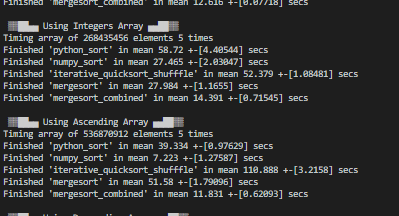
\includegraphics[scale=0.8]{output_to_terminal.PNG}
    \caption{Terminal output}
    \label{fig:outputterminal}
\end{figure}

\begin{table}
  % Table captions always come *above* the table.
  \caption{5 Random samples from results}
  \label{tab:DF}
\begin{tabular}{ |p{2cm}||p{0.5cm}|p{2cm}|p{2cm}|  }
 \hline
 \multicolumn{4}{|c|}{Results DataFrame} \\
 \hline
 Algorithm & $2^N$ & TypeArray & Time \\
 \hline
 \texttt{\detokenize{python_sort}}&15&Integers& 0.003036\\
 \texttt{\detokenize{numpy_sort}}&21  & Descending & 0.028119\\
  \texttt{\detokenize{numpy_sort}}&1 & Structured& 0.000002\\
 \texttt{\detokenize{numpy_sort}}&15 & Random& 0.002030\\
 \texttt{merge sort}&15& Structured& 0.002981\\
 \hline
\end{tabular}
\end{table}

\begin{table}
  % Table captions always come *above* the table.
  \caption{Versions of files used for this report; GitLab repository: \url{https://gitlab.com/nmbu.no/emner/inf221/h2020/student-term-papers/team_19/inf221-term-paper-team19}.}
  \label{tab:hashes}
  \begin{tabular}{ll}
    \hline
    File & Git hash THIS IS JUST A PLACEHOLDER ATM \\\hline
    \verb!utility.py! & \verb!8ec07210f! \\
    \verb!src! & \verb!396d8a309! \\
    \verb!plot_creation.ipynb! & \verb!8ec07210f! \\
    \verb!benchmark_results.csv! & \verb!88c28d55c! \\\hline
  \end{tabular}
\end{table}

\subsection{Challenges}\label{sec:challenges}

\begin{itemize}
\item Time taken to bench algorithms.
\item Quick sort is problematic with standard implementation. This caused recursion limits and made it difficult to plot against other algorithms. 
\item Threshold for merge sort combined.
\item Verifying the functionality of the sorting algorithms

\end{itemize}

\subsection{Solutions}\label{sec:solutions}
\begin{itemize}
\item JIT-compiled sorting algorithms (effect only on the first calls to the algorithms.) object-mode, beats even Numpy sort at certain problems. Could have compiled ahead of time, but since that causes implication with datatypes and what OS or Hardware you are running, we decided to compile Just in time with object mode. 
\item Implemented iterative quick sort with median of three partitioning 
\item Found the largest $\frac{\delta(a, b)}{\delta(n)}$ where a is time taken by merge sort and b is insertion sort. Which in our case was a threshold of 142, hence each split of merge sort with n < threshold is sorted using insertion sort.
\item Unittests in tests/test\_algos.py

\end{itemize}

\section{Results}\label{sec:results}

The first two algorithms we compared were the quadratic sorting algorithms shown in figure~\ref{fig:bubble_insertion}. Insertion sort clearly performs better for all types of arrays except for ascending arrays. \newline

Comparing merge sort and insertion sort \dots

The next two algorithms we compared were the sub-quadratic algorithms. As we can see in figure~\ref{fig:merge_quick}, quick sort performs better than merge sort when sorting all arrays up to a certain size. For ascending and descending arrays quick sorts performs the best for all array sizes. However, quick sorts performance also varies a lot depending on the type of the arrays. Merge sort on the other hand, stays surprisingly stable in performance when both the type and size of the array varies. When the array size approaches a length of $2^(28)$ and greater, both the algorithms seem to struggle. \newline

We then moved on to compare merge sort with merge sort combined, seen in figure~\ref{fig:merge_mergecomb}. Both algorithms have a similar decrease in performance as the array size increases along the x-axis. However merge sort combined clearly performs better than ordinary merge sort when it comes to all the array types. Another difference is that merge sort combined's performance is less stable across the types of arrays. It sorts ascending arrays the best, then integers and structured arrays and so on. Whereas ordinary merge sort performs quite similarly time wise on all array types. In this plot as well there seems to be a struggle when the array size exceeds a length of $2^{28}$. \newline

Finally we decided to compare our best performer, merge sort combined, with NumPy and Python's in place sort. From figure~\ref{fig:np_py_mergecomb} it is harder to make a definite conclusion at a first glance, however when looking closely one can see that merge sort combined still is the most stable across all types of arrays and also as array size increases. In addition it beats both the other two algorithms in random, structured and integer arrays. Although, NumPy sort is clearly superior when it comes to ascending and descending arrays. \newline

\begin{figure}[]
  \centering
  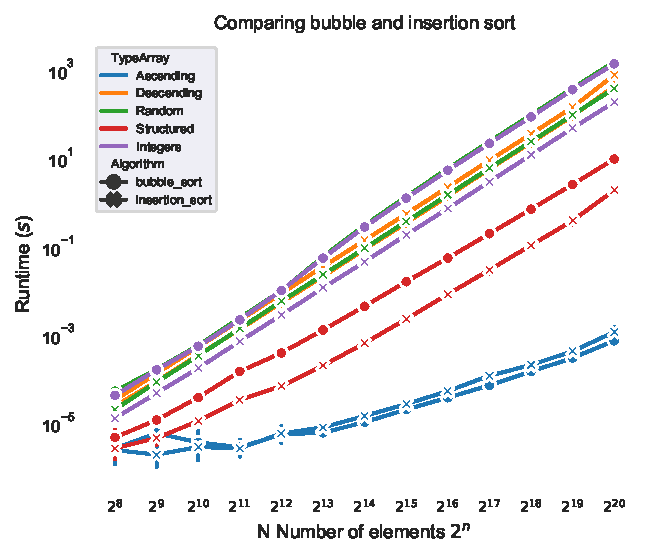
\includegraphics[scale=0.85]{runtimebubble&insertion.pdf}
  % figure captions below figure
  \caption{Benchmark results for insertion sort and bubble sort.}
  \label{fig:bubble_insertion}
\end{figure}

\begin{figure}[]
  \centering
  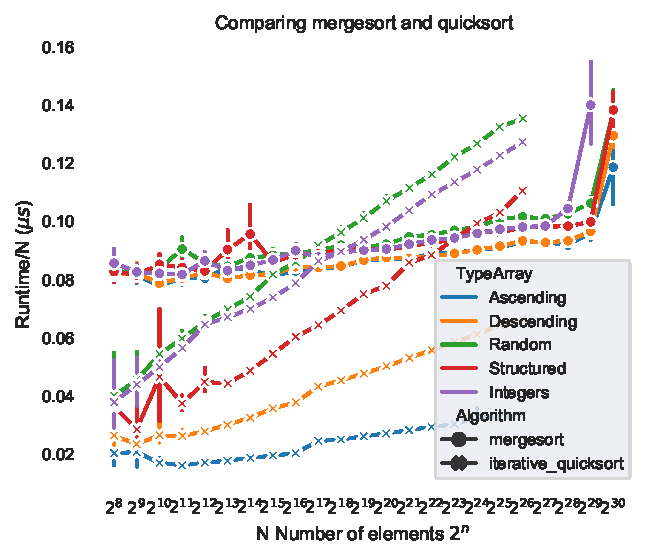
\includegraphics[scale=0.85]{runtime_per_n_merge&quick.pdf}
  % figure captions below figure
  \caption{Benchmark results for merge sort and quick sort.}
  \label{fig:merge_quick}
\end{figure}

\begin{figure}[]
  \centering
  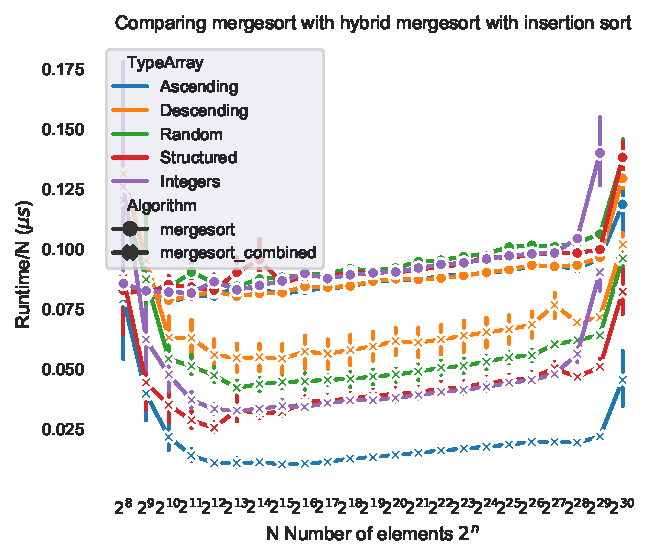
\includegraphics[scale=0.85]{runtime_per_n_merge&combined.pdf}
  % figure captions below figure
  \caption{Benchmark results for merge sort and merge sort combined.}
  \label{fig:merge_mergecomb}
\end{figure}

\begin{figure}[]
  \centering
  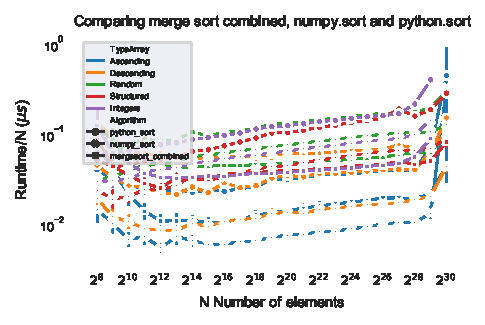
\includegraphics[scale=0.85]{INF221/runtime_per_n_combined&np&py.pdf}
  % figure captions below figure
  \caption{Benchmark results for merge sort combined, NymPy sort, and Python sort.}
  \label{fig:np_py_mergecomb}
\end{figure}

\section{Discussion}\label{sec:discussion}

As seen in the results, insertion sort performs better than bubble sort. This supports what we expected and explained in the theory section ~\ref{sec:algo2}. \newline

Even though there are many more powerful algorithms than insertion sort, such as merge sort, the time cost caused by their recursive implementation results in them failing to beat insertion sort when sorting small arrays. This is why insertion sort often is used internally in other sorting algorithms, to sort small portions of the input array, resulting in even better performing hybrid algorithms. Such as timsort or merge sort combined.

In figure ~\ref{fig:merge_quick} we saw that quick sort performs the best on ascending and descending lists. In theory section~\ref{sec:algo4} we mentioned that these arrays were the worst case scenario for quick sort. To handle this we used the 'median of three' implementation, which clearly has been effective in doing so. \newline

As mentioned in the results, the algorithms 'struggled' towards the end of the plots. Meaning they increased in runtime by a factor between 10 and 100 as the array size reached a length of $2^{29}$ to $2^{30}$ on the x-axis. This is because the RAM of the simulation computer is filled, and the memory is then shifted between physical memory and virtual memory, while dumping and collecting to and from storage temporarily. 

% In the acks section, you can thank people for help.
\begin{acks}
We are grateful to Kharikton Gurbatsjnov for guidance in calculating time savings.

\end{acks}

%% The next two lines define the bibliography style to be used, and
%% the bibliography file.
\bibliographystyle{ACM-Reference-Format}


%%% This doesnt work, tror vi trenger den bib fila
\begin{thebibliography}{References}


\bibitem{Iterative Quick Sort - GeeksforGeeks. 2020. GeeksforGeeks. https://www.geeksforgeeks.org/iterative-quick-sort/?fbclid=IwAR2ziWGZKt7nrgiD94kKu2if00gLmh3j2oNR6DUnSsL2b1AoLMsjvpARgYk.}
\bibitem[]{Insertion sort. 2020. En.wikipedia.org. https://en.wikipedia.org/wiki/Insertion_sort.}
\bibitem[]{Comparison of Sorting Algorithms. 2020. Medium. https://medium.com/@tssovi/comparison-of-sorting-algorithms-298fdf037c8f.}
\bibitem[]{Random Generator. 2020. NumPy. https://numpy.org/doc/stable/reference/random/generator.html#numpy.random.default_rng}
\bibitem[]{CLRS_2009,
 author = {Cormen, Thomas H. and Leiserson, Charles E. and Rivest, Ronald L. and Stein, Clifford},
 title = {Introduction to Algorithms, Third Edition},
 year = {2009},
 isbn = {0262033844, 9780262033848},
 edition = {3rd},
 publisher = {The MIT Press},
 address = {Cambridge, MA}}

\end{thebibliography}
%%%


\bibliography{References
Iterative Quick Sort - GeeksforGeeks. 2020. GeeksforGeeks. https://www.geeksforgeeks.org/iterative-quick-sort/?fbclid=IwAR2ziWGZKt7nrgiD94kKu2if00gLmh3j2oNR6DUnSsL2b1AoLMsjvpARgYk.}
\bibliography{Insertion sort. 2020. En.wikipedia.org. https://en.wikipedia.org/wiki/Insertion_sort.}
\bibliography{Comparison of Sorting Algorithms. 2020. Medium. https://medium.com/@tssovi/comparison-of-sorting-algorithms-298fdf037c8f.}
\bibliography{Random Generator. 2020. NumPy. https://numpy.org/doc/stable/reference/random/generator.html#numpy.random.default_rng}


\end{document}
